\section*{5 Programming Exercise (20 pts)}
\subsection*{5.1 Tensor Flow Playground for Neural Networks [5 pts]}
In this problem we will use the TensorFlow playground \href{http://playground.tensorflow.org}{http://playground.tensorflow.org}, which is a nice visual tool for training simple Multi Layer Perceptrons (MLPs).
Your goal in this problem is to carefully select input features to design the ``smallest'' MLP classifiers that can achieve low test loss for each of the 4 datasets in TensorFlow playground (Figures 1 - 4 show the 4 datasets available on TensorFlow playground). Note that you have to design a separate classifier for each individual dataset.  Here \emph{smallest} is defined as having least number of neurons in the network. By low test loss we mean a test loss $< 0.1$ for the swiss roll dataset and a test loss of $\approx 0$ for the rest of the datasets. Submit screenshots after your networks achieve the required test loss for each of the datasets.

\begin{figure}[!htb]
\minipage{0.23\textwidth}
  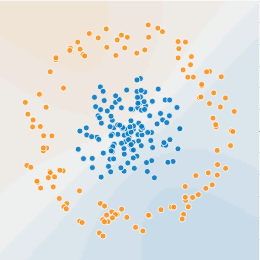
\includegraphics[width=\linewidth]{plots/Circles}
  \caption{Circles}\label{}
\endminipage\hfill
\minipage{0.23\textwidth}
  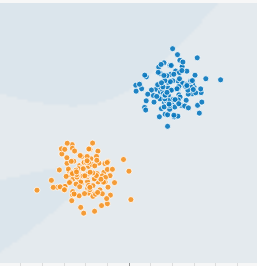
\includegraphics[width=\linewidth]{plots/Clusters}
  \caption{Clusters}\label{}
\endminipage\hfill
\minipage{0.23\textwidth}
  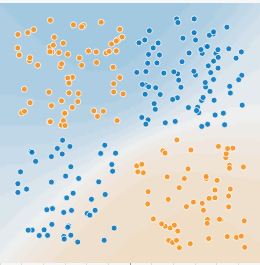
\includegraphics[width=\linewidth]{plots/Squares}
  \caption{Squares}\label{}
\endminipage\hfill
\minipage{0.23\textwidth}
  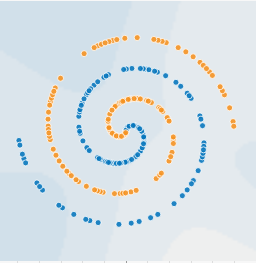
\includegraphics[width=\linewidth]{plots/SwissRoll}
  \caption{Swiss Roll}\label{}
\endminipage
\end{figure}

\begin{soln}
        % Type solution here
\end{soln}



\subsection*{5.2 Binary Classification [15pts]}
In this problem you will be using a binary (two class) version of \emph{mnist} dataset. The data and code template can be downloaded from Piazza Resources as \texttt{HW3\_Q5\_Data.zip}.

We use the following formulation in this problem:
\[
\min_{w\in \mathbb{R}^d}   \frac{\lambda}{2} \|w\|^2_2 + \frac{1}{n}\sum_{i = 1}^n \max(1 - y_i\left\langle w, X_i\right\rangle, 0).
\]
This is only done to simplify calculations. You will optimize this objective using Stochastic Sub-Gradient Descent (SSGD) (Shalev et. al., 2011). This approach is very simple and scales well to large datasets\footnote{To estimate optimal $w$, one can also optimize the dual formulation of this problem. Some of the popular SVM solvers such as LIBSVM solve the dual problem. Other fast approaches for solving dual formulation on large datasets use dual coordinate descent.}. In SSGD we randomly sample a training data point in each iteration and update the weight vector by taking a small step along the direction of negative ``sub-gradient'' of the loss\footnote{Sub-gradient generalizes the notion of gradient to non-differentiable  functions}. \pagebreak

The SSGD algorithm is given by:
\begin{itemize}
\item Initialize the weight vector $w = 0$.
\item For t = 1 \dots T 
\begin{itemize}
\item[*] Choose $i_t \in \{1, \dots n\}$ uniformly at random
\item[*] Set $\eta_t = \frac{1}{\lambda t}$.
\item[*] If $y_{i_t}\left\langle w, X_{i_t}\right\rangle < 1$ then:
\begin{itemize}
\item[--] Set $w \leftarrow (1- \lambda\eta_t)w + \eta_ty_{i_t}X_{i_t}$
\end{itemize}
\item[*] Else:
\begin{itemize}
\item[--] Set $w \leftarrow (1- \lambda\eta_t)w$
\end{itemize}
\end{itemize}
\item Return $w$
\end{itemize}
Note that we don't consider the bias/intercept term in this problem. 

\begin{itemize}
\item Complete the \texttt{train(w0, Xtrain, ytrain, T, lambda)} function in the \texttt{svm.py} file (\textttt{matlab} users complete the \textfff{train.m} file).
\begin{itemize}

\item The function \texttt{train(w0, Xtrain, ytrain, T, lambda)} runs the SSGD algorithm, taking in an initial weight vector \texttt{w0}, matrix of covariates \texttt{Xtrain}, a vector of labels \texttt{ytrain}. \texttt{T} is the number of iterations of SSGD and \texttt{lambda} is the hyper-parameter in the objective. It outputs the learned weight vector \texttt{w}.
\end{itemize}
\item Run \texttt{svm\_run.py} to perform training and see the performance on training and test sets.
\end{itemize}

\paragraph{Evaluation}
\begin{itemize}
\item Use \texttt{validation}  dataset for picking a good \texttt{lambda($\lambda$)} from the set \texttt{\{1e3, 1e2, 1e1, 1, 0.1\}}.
\item Report the accuracy numbers on train and test datasets obtained using the best \texttt{lambda}, after running SSGD for $200$ epochs (i.e., $T = 200*n$).  Generate the training accuracy vs. training time and test accuracy vs training time plots.
\end{itemize}

\begin{soln}
        % Type solution here
\end{soln}

